% !TEX root = calculus.tex

\chapter{LIMIT OF SEQUENCE}
\label{dialogue-02}
{\parindent=0pt
\athr What mathematical operations do you know?

\rdr Addition, subtraction, multiplication, division, involution (raising to a power), evolution (extracting n root), and taking a logarithm or a modulus.

\athr In order to pass from elementary mathematics to higher mathematics, this ``list'' should be supplemented with one more mathematical operation, namely, that of finding the limit of sequence; this operation is called sometimes the limit transition (or passage to the limit). By the way, we shall clarify below the meaning of the last phrase of the previous dialogue, stating that calculus ``begins'' where the limit of sequence is introduced. 

\rdr I heard that higher mathematics uses the operations of \emph{differentiation} and \emph{integration}. 

\athr These operations, as we shall see, are in essence nothing but the variations of the limit transition. 

Now, let us get down to the concept of the \emph{limit of sequence}. Do you know what it is? 

\rdr I learned the definition of the limit of sequence. However, I doubt that I can reproduce it from memory. 

\athr But you seem to ``feel'' this notion somehow? Probably, you can indicate which of the sequences discussed above have limits and what the value of the limit is in each case. 

\rdr I think I can do this, The limit is 1 for sequence \eqref{series-05}, zero for \eqref{series-07} and \eqref{series-09}, and $\pi$ for \eqref{series-13}. 

\athr That's right. The remaining sequences have no limits.

\rdr By the way, sequence \eqref{series-09} is not monotonic \ldots

\athr Apparently, you have just remembered the end of our previous dialogue where it was stated that if a sequence is both monotonic and bounded, it has a limit.

\rdr That's correct. But isn't this a contradiction?

\athr Where do you find the contradiction? Do you think that from the statement ``If a sequence is both monotonic and bounded, it has a limit'' one should necessarily draw a reverse statement like ``If a sequence has a limit, it must be monotonic and bounded?'' Later we shall see that a necessary condition for a limit is only the boundedness of a sequence. The monotonicity is not mandatory at all; consider, for example, sequence \eqref{series-09}.

Let us get back to the concept of the limit of sequence. Since you have correctly indicated the sequences that have limits, you obviously have some understanding of this concept. Could you formulate it?

\rdr A limit is a number to which a given sequence tends (converges).

\athr What do you mean by saying ``converges to a number''?

\rdr I mean that with an increase of the serial number, the terms of a sequence converge very closely to a certain value.

\athr What do you mean by saying ``very closely''?

\rdr Well, the ``difference'' between the values of the terms and the given number will become infinitely small. Do you think any additional explanation is needed?

\athr The definition of the limit of sequence which you have suggested can at best be classified as a subjective impression. We have already discussed a similar situation in the previous dialogue.

Let us see what is hidden behind the statement made above. For this purpose, let us look at a rigorous definition of the limit of sequence which we are going to examine in detail.
\begin{mytheo}{Definition}
The number $a$ is said to be the limit of sequence ($y_{n}$) if for any positive number $\varepsilon$ there is a real number $N$ such that for all $ n > N$ the following inequality holds:
\begin{equation}%
| \, y_{n} - a \, | < \varepsilon
\label{limit-of-seq}
\end{equation}
\end{mytheo}

\rdr I am afraid, it is beyond me to remember such a definition.

\athr Don't hasten to remember. Try to comprehend this definition, to realize its structure and its inner logic. You will see that every word in this phrase carries a definite and necessary content and that no other definition of the limit of sequence could be more succinct (more delicate, even). 

First of all, let us note the logic of the sentence. A certain number is the limit provided that for any $\varepsilon > 0$ \emph{there is} a number $N$ such that for all $n > N$ inequality \eqref{limit-of-seq} holds. In short, it is necessary that for any $\varepsilon$ a certain number $N$ should exist.

Further, note two ``delicate'' aspects in this sentence. First, the number $N$ should exist for any positive number $\varepsilon$. Obviously, \emph{there is} an infinite set of such $\varepsilon$. Second, inequality \eqref{limit-of-seq} should hold always (i.e. for each $\varepsilon$) for \emph{all} $n > N$. But there is an equally infinite set of numbers n!

\rdr Now, the definition of the limit has become more obscure.

\athr Well, it is natural. So far we have been examining the definition ``piece by piece''. It is very important that the ``delicate'' features, the ``cream'', so to say, are spotted from the very outset. Once you understand them, everything will fall into place.

In \fig{fig-07}\textcolor{IndianRed}{(a)} there is a graphic image of a sequence. Strictly speaking, the first 40 terms have been plotted on the graph. Let us assume that if any regularity is noted in these 40 terms, we shall conclude that the regularity does exist for $n > 40$.

\begin{figure}[!h]
\centering
{\noindent
\begin{tikzpicture}[line cap=round,line join=round,>=triangle 45,x=0.2cm,y=0.3cm]
\foreach \x in {0,10,20,30,40}
\draw[shift={(\x,-4)},color=black] (0pt,2pt) -- (0pt,-2pt) node[below] {\footnotesize $\x$};
%\draw[color=black] (0pt,-10pt) node[right] {\footnotesize $0$};
\clip(-5.5,-6) rectangle (52,6);
\foreach \x in {1,...,40}
\draw [line width=.75pt,dash pattern=on 5pt off 5pt,color=DarkGray] (\x,4.)-- (\x,-4.);

\draw [line width=1pt,dash pattern=on 3pt off 3pt,color=IndianRed] (0.,0.)-- (42.,0.);
\draw [->,line width=1.2pt,color=DarkGray] (0.,-4.) -- (0.,5.348012295333778);
\draw [->,line width=1.2pt,color=DarkGray] (0.,-4.) -- (50,-4.);
\draw (-.5,4.5) node[left] {\footnotesize$y_{n}$};
\draw (0,0) node[left] {\footnotesize$a$};
\draw (48,-4.028170894118617) node[below] {\footnotesize$n$};
\begin{scriptsize}
\draw (-2.8,-4) node[left] {\normalsize \textit{ (a)}};
\filldraw [IndianRed] (0.,0.) circle (1.5pt);
\filldraw [IndianRed] (1.,-3.24098) circle (1.5pt);
\filldraw [IndianRed] (2.,3.49351) circle (1.5pt);
\filldraw [IndianRed] (3.,-3.24098) circle (1.5pt);
\filldraw [IndianRed] (4.,1.92) circle (1.5pt);
\filldraw [IndianRed] (5.,0.) circle (1.5pt);
\filldraw [IndianRed] (6.,2.84361) circle (1.5pt);
\filldraw [IndianRed] (7.,-3.1191) circle (1.5pt);
\filldraw [IndianRed] (8.,2.53306) circle (1.5pt);
\filldraw [IndianRed] (9.,-2.5808) circle (1.5pt);
\filldraw [IndianRed] (10.,1.19082) circle (1.5pt);
\filldraw [IndianRed] (11.,2.11898) circle (1.5pt);
\filldraw [IndianRed] (13.,2.05687) circle (1.5pt);
\filldraw [IndianRed] (12.,-2.97418) circle (1.5pt);
\filldraw [IndianRed] (14.053794841260318,-1.0487146075110734) circle (1.5pt);
\filldraw [IndianRed] (16.,1.04238) circle (1.5pt);
\filldraw [IndianRed] (15.,-1.87687) circle (1.5pt);
\filldraw [IndianRed] (17.,-1.66983) circle (1.5pt);
\filldraw [IndianRed] (18.,-0.59323) circle (1.5pt);
\filldraw [IndianRed] (19.,0.) circle (1.5pt);
\filldraw [IndianRed] (20.,1.39434) circle (1.5pt);
\filldraw [IndianRed] (21.,0.77323) circle (1.5pt);
\filldraw [IndianRed] (22.,-1.54561) circle (1.5pt);
\filldraw [IndianRed] (23.,-0.67604) circle (1.5pt);
\filldraw [IndianRed] (24.,0.56619) circle (1.5pt);
\filldraw [IndianRed] (25.,1.35294) circle (1.5pt);
\filldraw [IndianRed] (26.,0.) circle (1.5pt);
\filldraw [IndianRed] (27.,-1.06942) circle (1.5pt);
\filldraw [IndianRed] (28.,0.52478) circle (1.5pt);
\filldraw [IndianRed] (29.,-0.51041) circle (1.5pt);
\filldraw [IndianRed] (30.,-0.51041) circle (1.5pt);
\filldraw [IndianRed] (31.,0.46267) circle (1.5pt);
\filldraw [IndianRed] (32.,0.44196) circle (1.5pt);
\filldraw [IndianRed] (33.,0.71112) circle (1.5pt);
\filldraw [IndianRed] (34.,-0.51041) circle (1.5pt);
\filldraw [IndianRed] (35.,0.25563) circle (1.5pt);
\filldraw [IndianRed] (36.,0.29704) circle (1.5pt);
\filldraw [IndianRed] (37.,-0.05493) circle (1.5pt);
\filldraw [IndianRed] (38.,-0.48971) circle (1.5pt);
\filldraw [IndianRed] (39.,0.25563) circle (1.5pt);
\filldraw [IndianRed] (40.,0.25563) circle (1.5pt);
\end{scriptsize}
\end{tikzpicture}
% part 2
\begin{tikzpicture}[line cap=round,line join=round,>=triangle 45,x=0.2cm,y=0.3cm]
\foreach \x in {0,10,20,30,40}
\draw[shift={(\x,-4)},color=black] (0pt,2pt) -- (0pt,-2pt) node[below] {\footnotesize $\x$};
%\draw[color=black] (0pt,-10pt) node[right] {\footnotesize $0$};
\clip(-5.5,-6) rectangle (52,6);
\foreach \x in {1,...,40}
\draw [line width=.75pt,dash pattern=on 5pt off 5pt,color=DarkGray] (\x,4.)-- (\x,-4.);
\draw [line width=.5pt,dash pattern=on 5pt off 5pt,color=DodgerBlue] (0.,2.8)-- (44.,2.8);
\draw [line width=.5pt,dash pattern=on 5pt off 5pt,color=DodgerBlue] (0.,-2.8)-- (44.,-2.8);
\draw [<->,line width=.75pt,color=DarkGray] (43,2.8)-- (43,-2.8);
\draw (43,0) node[right,color=black] {\footnotesize $2 \varepsilon$};
\draw (0.,2.8) node[left,color=black] {\footnotesize $a + \varepsilon$};
\draw (0.,-2.8) node[left,color=black] {\footnotesize $a - \varepsilon$};
\draw [line width=1pt,dash pattern=on 3pt off 3pt,color=IndianRed] (0.,0.)-- (42.,0.);
\draw [->,line width=1.2pt,color=DarkGray] (0.,-4.) -- (0.,5.348012295333778);
\draw [->,line width=1.2pt,color=DarkGray] (0.,-4.) -- (50,-4.);
\draw (-.5,4.5) node[left] {\footnotesize $y_{n}$};
\draw (0,0) node[left] {\footnotesize $a$};
\draw (48,-4) node[below] {\footnotesize $n$};
\begin{scriptsize}
\draw (-2.8,-4) node[left] {\normalsize \textit{(b)}};
\filldraw [IndianRed] (0.,0.) circle (1.5pt);
\filldraw [IndianRed] (1.,-3.24098) circle (1.5pt);
\filldraw [IndianRed] (2.,3.49351) circle (1.5pt);
\filldraw [IndianRed] (3.,-3.24098) circle (1.5pt);
\filldraw [IndianRed] (4.,1.92) circle (1.5pt);
\filldraw [IndianRed] (5.,0.) circle (1.5pt);
\filldraw [IndianRed] (6.,2.84361) circle (1.5pt);
\filldraw [IndianRed] (7.,-3.1191) circle (1.5pt);
\filldraw [IndianRed] (8.,2.53306) circle (1.5pt);
\filldraw [IndianRed] (9.,-2.5808) circle (1.5pt);
\filldraw [IndianRed] (10.,1.19082) circle (1.5pt);
\filldraw [IndianRed] (11.,2.11898) circle (1.5pt);
\filldraw [IndianRed] (13.,2.05687) circle (1.5pt);
\filldraw [IndianRed] (12.,-2.97418) circle (1.5pt);
\filldraw [IndianRed] (14.053794841260318,-1.0487146075110734) circle (1.5pt);
\filldraw [IndianRed] (16.,1.04238) circle (1.5pt);
\filldraw [IndianRed] (15.,-1.87687) circle (1.5pt);
\filldraw [IndianRed] (17.,-1.66983) circle (1.5pt);
\filldraw [IndianRed] (18.,-0.59323) circle (1.5pt);
\filldraw [IndianRed] (19.,0.) circle (1.5pt);
\filldraw [IndianRed] (20.,1.39434) circle (1.5pt);
\filldraw [IndianRed] (21.,0.77323) circle (1.5pt);
\filldraw [IndianRed] (22.,-1.54561) circle (1.5pt);
\filldraw [IndianRed] (23.,-0.67604) circle (1.5pt);
\filldraw [IndianRed] (24.,0.56619) circle (1.5pt);
\filldraw [IndianRed] (25.,1.35294) circle (1.5pt);
\filldraw [IndianRed] (26.,0.) circle (1.5pt);
\filldraw [IndianRed] (27.,-1.06942) circle (1.5pt);
\filldraw [IndianRed] (28.,0.52478) circle (1.5pt);
\filldraw [IndianRed] (29.,-0.51041) circle (1.5pt);
\filldraw [IndianRed] (30.,-0.51041) circle (1.5pt);
\filldraw [IndianRed] (31.,0.46267) circle (1.5pt);
\filldraw [IndianRed] (32.,0.44196) circle (1.5pt);
\filldraw [IndianRed] (33.,0.71112) circle (1.5pt);
\filldraw [IndianRed] (34.,-0.51041) circle (1.5pt);
\filldraw [IndianRed] (35.,0.25563) circle (1.5pt);
\filldraw [IndianRed] (36.,0.29704) circle (1.5pt);
\filldraw [IndianRed] (37.,-0.05493) circle (1.5pt);
\filldraw [IndianRed] (38.,-0.48971) circle (1.5pt);
\filldraw [IndianRed] (39.,0.25563) circle (1.5pt);
\filldraw [IndianRed] (40.,0.25563) circle (1.5pt);
\end{scriptsize}
\end{tikzpicture}
% part 3
\begin{tikzpicture}[line cap=round,line join=round,>=triangle 45,x=0.2cm,y=0.3cm]
\foreach \x in {0,10,20,30,40}
\draw[shift={(\x,-4)},color=black] (0pt,2pt) -- (0pt,-2pt) node[below] {\footnotesize $\x$};
%\draw[color=black] (0pt,-10pt) node[right] {\footnotesize $0$};
\clip(-5.5,-6) rectangle (52,6);
\foreach \x in {1,...,40}
\draw [line width=.75pt,dash pattern=on 5pt off 5pt,color=DarkGray] (\x,4.)-- (\x,-4.);
\draw [line width=1pt,dash pattern=on 3pt off 3pt,color=IndianRed] (0.,0.)-- (42.,0.);
\draw [->,line width=1.2pt,color=DarkGray] (0.,-4.) -- (0.,5.348012295333778);
\draw [->,line width=1.2pt,color=DarkGray] (0.,-4.) -- (50,-4.);
\draw (-.5,4.5) node[left] {\footnotesize$y_{n}$};
\draw (0,0) node[left] {\footnotesize$a$};
\draw [line width=.5pt,dash pattern=on 5pt off 5pt,color=DodgerBlue] (7.,2)-- (50.,2);
\draw [line width=.5pt,dash pattern=on 5pt off 5pt,color=DodgerBlue] (7.,-2)-- (50.,-2);
\draw [line width=.5pt,dash pattern=on 5pt off 5pt,color=DodgerBlue] (15.,1.2)-- (47.,1.2);
\draw [line width=.5pt,dash pattern=on 5pt off 5pt,color=DodgerBlue] (15.,-1.2)-- (47.,-1.2);
\draw [line width=.5pt,dash pattern=on 5pt off 5pt,color=DodgerBlue] (27.,.5)-- (43.,.5);
\draw [line width=.5pt,dash pattern=on 5pt off 5pt,color=DodgerBlue] (27.,-.5)-- (43.,-.5);
\draw (48,-4.028170894118617) node[below] {\footnotesize$n$};
\draw [<->,line width=.75pt,color=DarkGray] (49,2)-- (49,-2);
\draw [<->,line width=.75pt,color=DarkGray] (46,1.2)-- (46,-1.2);
\draw (49,0) node[right,color=black] {\footnotesize $2 \varepsilon_{1}$};
\draw (46,0) node[right,color=black] {\footnotesize $2 \varepsilon_{2}$};
\draw (42,0) node[right,color=black] {\footnotesize $2 \varepsilon_{3}$};
\begin{scriptsize}
\draw (-2.8,-4) node[left] {\normalsize \textit{(c)}};
\filldraw [IndianRed] (0.,0.) circle (1.5pt);
\filldraw [IndianRed] (1.,-3.24098) circle (1.5pt);
\filldraw [IndianRed] (2.,3.49351) circle (1.5pt);
\filldraw [IndianRed] (3.,-3.24098) circle (1.5pt);
\filldraw [IndianRed] (4.,1.92) circle (1.5pt);
\filldraw [IndianRed] (5.,0.) circle (1.5pt);
\filldraw [IndianRed] (6.,2.84361) circle (1.5pt);
\filldraw [IndianRed] (7.,-3.1191) circle (1.5pt);
\filldraw [IndianRed] (8.,2.53306) circle (1.5pt);
\filldraw [IndianRed] (9.,-2.5808) circle (1.5pt);
\filldraw [IndianRed] (10.,1.19082) circle (1.5pt);
\filldraw [IndianRed] (11.,2.11898) circle (1.5pt);
\filldraw [IndianRed] (13.,2.05687) circle (1.5pt);
\filldraw [IndianRed] (12.,-2.97418) circle (1.5pt);
\filldraw [IndianRed] (14.053794841260318,-1.0487146075110734) circle (1.5pt);
\filldraw [IndianRed] (16.,1.04238) circle (1.5pt);
\filldraw [IndianRed] (15.,-1.87687) circle (1.5pt);
\filldraw [IndianRed] (17.,-1.66983) circle (1.5pt);
\filldraw [IndianRed] (18.,-0.59323) circle (1.5pt);
\filldraw [IndianRed] (19.,0.) circle (1.5pt);
\filldraw [IndianRed] (20.,1.39434) circle (1.5pt);
\filldraw [IndianRed] (21.,0.77323) circle (1.5pt);
\filldraw [IndianRed] (22.,-1.54561) circle (1.5pt);
\filldraw [IndianRed] (23.,-0.67604) circle (1.5pt);
\filldraw [IndianRed] (24.,0.56619) circle (1.5pt);
\filldraw [IndianRed] (25.,1.35294) circle (1.5pt);
\filldraw [IndianRed] (26.,0.) circle (1.5pt);
\filldraw [IndianRed] (27.,-1.06942) circle (1.5pt);
\filldraw [IndianRed] (28.,0.52478) circle (1.5pt);
\filldraw [IndianRed] (29.,-0.51041) circle (1.5pt);
\filldraw [IndianRed] (30.,-0.51041) circle (1.5pt);
\filldraw [IndianRed] (31.,0.46267) circle (1.5pt);
\filldraw [IndianRed] (32.,0.44196) circle (1.5pt);
\filldraw [IndianRed] (33.,0.71112) circle (1.5pt);
\filldraw [IndianRed] (34.,-0.51041) circle (1.5pt);
\filldraw [IndianRed] (35.,0.25563) circle (1.5pt);
\filldraw [IndianRed] (36.,0.29704) circle (1.5pt);
\filldraw [IndianRed] (37.,-0.05493) circle (1.5pt);
\filldraw [IndianRed] (38.,-0.48971) circle (1.5pt);
\filldraw [IndianRed] (39.,0.25563) circle (1.5pt);
\filldraw [IndianRed] (40.,0.25563) circle (1.5pt);
\end{scriptsize}
\end{tikzpicture}
}
%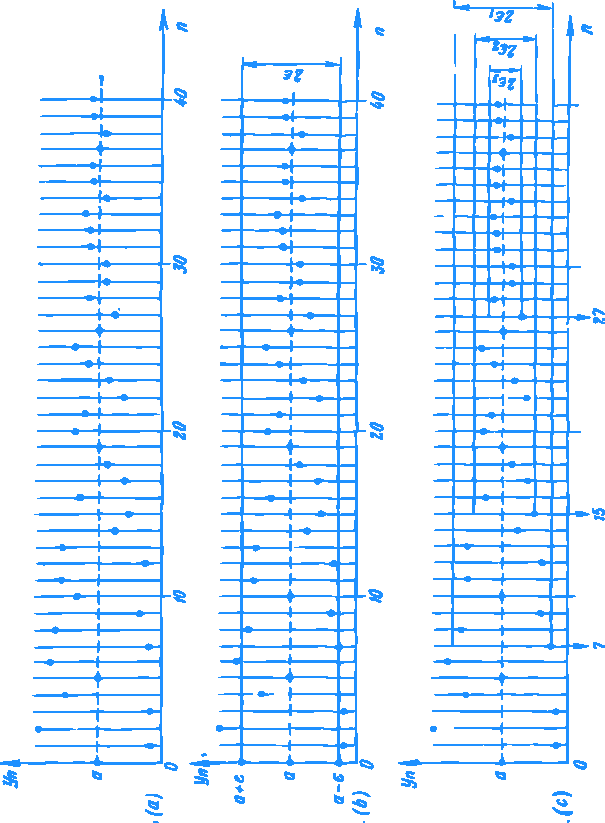
\includegraphics[width=0.9\textwidth]{figures/fig-07.pdf}
\caption{Finding limit of a sequence.}
\label{fig-07}
\end{figure}

Can we say that this sequence converges to the number $a$ (in other words, the number $a$ is the limit of the sequence)?

\rdr It seems plausible.

\athr Let us however, act not on the basis of our impressions but on the basis of the definition of the limit of sequence. So, we want to verify whether the number $a$ is the limit of the given sequence. What does our definition of the limit prescribe us to do?

\rdr We should take a positive number $\varepsilon$. 

\athr Which number? 

\rdr Probably. it must be small enough,

\athr The words ``small enough'' are neither here nor there. The number $\varepsilon$ must be arbitrary.

Thus, we take an arbitrary positive $\varepsilon$. Let us have a look at  \fig{fig-07}and layoff on the $y$-axis an interval of length $\varepsilon$, both upward and downward from the same point $a$. Now, let us draw through the points $y = a + \varepsilon$ and $y = a - \varepsilon$ the horizontal straight lines that mark an ``allowed'' band for our sequence. If for any term of the sequence inequality \eqref{limit-of-seq} holds, the points on the graph corresponding to these terms fall inside the ``allowed'' band. We see  in \fig{fig-07}\textcolor{IndianRed}{(b)} that starting from number $\varepsilon$, all the terms of the sequence stay within the limits of the ``allowed'' band, proving the validity of \eqref{limit-of-seq} for these terms. We, of course, assume that this situation will realize for all $n > 40$, i.e. for the whole infinite ``tail'' of the sequence not shown in the diagram.

Thus, for the selected $\varepsilon$ the number $N$ does exist. In this particular case we found it to be 7.


\rdr Hence, we can regard $a$ as the limit of the sequence.

\athr Don't you hurry. The definition clearly emphasizes: ``for \emph{any} positive $\varepsilon$''. So far we have analyzed only one value of $\varepsilon$. We should take another value of $\varepsilon$ and find $N$ not for a larger but for a smaller $\varepsilon$. If for the second $\varepsilon$ the search of $N$ is a success, we should take a third, even smaller $\varepsilon$, and then a fourth, still smaller $\varepsilon$, etc., repeating each time the operation of finding $N$.

In   \fig{fig-07}\textcolor{IndianRed}{(c)} three situations are drawn up for  $\varepsilon_{1}, \varepsilon_{2}$and $\varepsilon_{3}$ (in this case $\varepsilon_{1} > \varepsilon_{2} > \varepsilon_{3}$). Correspondingly, three ``allowed'' bands are plotted on the graph. For a greater clarity, each of these bands has its own starting $N$. We have chosen $N_{1}=7, \, N_{2} =15$, and $N_{3}=27$. 

Note that for each selected $\varepsilon$ we observe the same situation in  \fig{fig-07}\textcolor{IndianRed}{(c)}: up to a certain $n$, the sequence, speaking figuratively, may be ``indisciplined'' (in other words, some terms may fallout of the limits of the corresponding ``allowed'' band). However, after a certain $n$ is reached, a very rigid law sets in, namely, \emph{all the remaining terms of the sequence} (their number is infinite) \emph{do stay within the band}.

\rdr Do we really have to check it for an infinite number of $\varepsilon$ values?

\athr Certainly not. Besides, it is impossible. We must be sure that \emph{whichever} value of $\varepsilon > 0$ we take, there is such $N$ after which the whole infinite ``tail'' of the sequence will get ``locked up'' within the limits of the corresponding ``allowed'' band.

\rdr And what if we are not so sure?

\athr If we are not and if one can find a value of $\varepsilon_{1}$ such that it is impossible to ``lock up'' the infinite ``tail'' of the sequence within the limits of its ``allowed'' hand, then a is not the limit of our sequence.

\rdr And when do we reach the certainty?

\athr We shall talk this matter over at a later stage because it has nothing to do with the essence of the definition of the limit of sequence.
I suggest that you formulate this definition anew. Don't try to reconstruct the wording given earlier, just try to put it in your own words.

\rdr I'll try. The number $a$ is the limit of a given sequence if for any positive $\varepsilon$ there is (one can find) a serial number $n$ such that for all subsequent numbers (i.e. for the whole infinite ``tail'' of the sequence) the following inequality holds: $| \, y_{n} - a \, | < \varepsilon$.

\athr Excellent. You have almost repeated word by word the definition that seemed to you impossible to remember.

\rdr Yes, in reality it all has turned out to be quite logical and rather easy.

\athr It is worthwhile to note that the dialectics of thinking was clearly at work in this case: a concept becomes ``not difficult'' because the ``complexities'' built into it were clarified. First, we break up the concept into fragments, expose the ``complexities'', then examine the ``delicate'' points, thus trying to reach the ``core'' of the problem. Then we recompose the concept to make it integral, and, as a result, this reintegrated concept becomes sufficiently simple and comprehensible. In the future we shall try first to find the internal structure and internal logic of the concepts and theorems.

I believe we can consider the concept of the limit of sequence as thoroughly analyzed. I should like to add that, as a result, the meaning of the sentence ``the sequence converges to $a$'' has been explained. I remind you that initially
this sentence seemed to you as requiring no additional explanations.

\rdr At the moment it does not seem so self-evident any more. True, I see 
now quite clearly the idea behind it.

\athr Let us get back to examples  \eqref{series-05}, \eqref{series-07}, and  \eqref{series-09}. Those are the sequences that we discussed at the beginning of our talk. To begin with, we note that the fact that a sequence ($y_{n}$) converges to a certain number $a$ is conventionally written as
\begin{equation*}%
\lim\limits_{n \to \infty} y_{n}= a	
\end{equation*}
(it reads like this: ``The limit of $y_{n}$ for $n$ tending to infinity is $a$.'')

Using the definition of the limit, let us prove that 
\begin{equation*}%
\begin{split}
\lim\limits_{n \to \infty} \dfrac{n}{n+1} = 1; \quad \lim\limits_{n \to \infty} \frac{1}{n}= 0;\\
\lim\limits_{n \to \infty} \left\{ \frac{1}{2n} [1 - (-1)^{n}] - \frac{1}{2(n-1)}  [1 + (-1)^{n}] \right\} =0
\end{split}
\end{equation*}
You will begin with the first of the above problems. 

\rdr I have to prove that
\begin{equation*}%
\lim\limits_{n \to \infty} \dfrac{n}{n+1} = 1
\end{equation*}
I choose an arbitrary value of $\varepsilon$, for example, $\varepsilon = 0.1$. 

\athr I advise you to begin with finding the modulus
of $| y_{n}- a|$. 

\rdr In this case, the-modulus is
\begin{equation*}%
\left| \dfrac{n}{n+1} - 1 \right| = \dfrac{1}{n+1} 
\end{equation*}

\athr Apparently $\varepsilon$ needn't be specified, at least at the beginning.

\rdr O.K. Therefore. for an arbitrary positive value of $\varepsilon$, I have to find $N$ such that for all $n > N$ the following inequality holds
\begin{equation*}%
\dfrac{1}{n+1} < \varepsilon
\end{equation*}

\athr Quite correct. Go on.

\rdr The inequality can be rewritten in the form t
\begin{equation*}%
n > \dfrac{1}{\varepsilon} - 1 
\end{equation*}
It follows that the unknown $N$ may be identified as an integral part of $\dfrac{1}{\varepsilon} -	1$. Apparently, for all $n > N$ the inequality in question will hold. 

\athr That's right. Let, for example, $\varepsilon = 0.01$. 

\rdr Then $N = \dfrac{1}{\varepsilon} - 1 = 100 - 1 = 99$.

\athr Let $\varepsilon  = 0.001$.

\rdr Then $N = \dfrac{1}{\varepsilon} - 1 = 1000 - 1 = 999$.

\athr Let $\varepsilon  = 0.00015$.

\rdr Then $N = \dfrac{1}{\varepsilon} - 1 = 6665$.

\athr It is quite evident that for any $\varepsilon$ (no matter how small) we can find a corresponding $N$.

As to proving that the limits of sequences \eqref{series-07} and \eqref{series-09} are zero, we shall leave it to the reader as an exercise.

\rdr But couldn't the proof of the equality $\lim\limits_{n \to \infty} \dfrac{n}{n+1} = 1$ be simplified?

\athr Have a try.

\rdr Well, first I rewrite the expression in the following way:
\begin{equation*}%
\lim\limits_{n \to \infty} \dfrac{n}{n+1} = \lim\limits_{n \to \infty} \dfrac{1}{\dfrac{1}{n+1}}
\end{equation*}
Then I take into consideration that with an increase in $n$, fraction $\dfrac{1}{n}$ will tend to zero, and, consequently, can be neglected against unity. Hence, we may reject $\dfrac{1}{n}$ and have:  $ \lim\limits_{n \to \infty} \dfrac{1}{1} = 1 $.

\athr In practice this is the method generally used. However	one should note that in this case we have assumed,
first, that $ \lim\limits_{n \to \infty} \dfrac{1}{n} = 0 $, and, second, the validity of the following rules
\begin{align}%
\lim\limits_{n \to \infty} \frac{x_{n}}{y_{n}} & = \frac{\lim\limits_{n \to \infty} x_{n}}{\lim\limits_{n \to \infty} y_{n}} \label{lim-div}\\
\lim\limits_{n \to \infty} (x_{n} + z_{n}) & =\lim\limits_{n \to \infty} x_{n} + \lim\limits_{n \to \infty} z_{n} \label{lim-sum}
\end{align} 
where $x_{n} =1, \, y_{n} = 1 + \dfrac{1}{n}$ and $z_{n} = \dfrac{1}{n}$. Later on we shall discuss these rules, but at this juncture I suggest that we simply use them to compute several limits. Let us discuss two examples.	

\textcolor{IndianRed}{\bf Example 1} Find $ \lim\limits_{n \to \infty} \dfrac{3n - 1}{5n - 6} $.

\rdr It will be convenient to present the computation in the form:
\begin{align*}%
\lim\limits_{n \to \infty} \dfrac{3n - 1}{5n - 6} & = \lim\limits_{n \to \infty} \dfrac{3 - \dfrac{1}{n}}{5 - \dfrac{6}{n}} \\
& = \dfrac{\lim\limits_{n \to \infty} \left(3 - \dfrac{1}{n}\right)}{\lim\limits_{n \to \infty} \left(5 - \dfrac{6}{n}\right)}
= \dfrac{3}{5}
\end{align*} 
\athr Ok. \textcolor{IndianRed}{\bf Example 2} Compute
\begin{equation*}%
\lim\limits_{n \to \infty} \dfrac{6n^{2} - 1}{5n^{2} +2n -1} 
\end{equation*}
\rdr We write
\begin{equation*}%
\lim\limits_{n \to \infty} \dfrac{6n^{2} - 1}{5n^{2} +2n -1}  = \lim\limits_{n \to \infty} \dfrac{6n - \dfrac{1}{n}}{5n +2 - \dfrac{1}{n}}.
\end{equation*}

\athr Wait a moment! Did you think about the reason for dividing both the numerator and denominator of the fraction in the previous example by $n$? We did this because sequences $(3 n - 1)$ and $(5n -	6)$	obviously have no limits, and therefore rule \eqref{lim-div} fails. However, each of
sequences $\left( 3 - \dfrac{1}{n} \right)$ and $\left( 5 - \dfrac{6}{n} \right)$ has a limit.

\rdr I have got your point. It means that in \textcolor{IndianRed}{\bf Example 2} I have to divide both the numerator and denominator by $n^{2}$ to obtain the sequences with limits in both. Accordingly we obtain
\begin{align*}%
\lim\limits_{n \to \infty} \dfrac{6n^{2} - 1}{5n^{2} +2n -1}  & = \lim\limits_{n \to \infty} \dfrac{6 - \dfrac{1}{n^{2}}}{5 + \dfrac{2}{n} - \dfrac{1}{n^{2}}} \\
& = \frac{\lim\limits_{n \to \infty} \left( 6 - \dfrac{1}{n^{2}}\right) }{\lim\limits_{n \to \infty} \left( 5 + \dfrac{2}{n	} - \dfrac{1}{n^{2}}\right)}
\end{align*}


\athr Well, we have examined the concept of the limit of sequence. Moreover, we have learned a little how to calculate limits. Now it is time to discuss some properties of sequences with limits. Such sequences are called \emph{convergent}.
}